Consider a task where we try to predict the last word in "The clouds are in the \textit{sky}". It is fairly obvious the last word is meant to be "\textit{sky}". The gap between the relevant information and the prediction place is small, and RNN can learn to utilize past information and predict the last word. However, if we consider "I grew up in Spain... I speak fluent \textit{Spanish}", the gap between the relevant information and predicting word can become large. As the gap grows, RNNs are unable to handle the task. Such problem is called \textit{long-term dependencies} \cite{colahLSTM}.

Long Short Term Memory networks (LSTM) are RNN architecture first introduced by Hochreiter S. and Schmidhuber J. \cite{hochreiterLSTM} with the ability to handle long-term dependencies. Its core idea is to replace RNN's hidden states with so-called \textbf{LSTM Cells} and add connections between cells, called \textit{cell states} or $c_{t}$. Each LSTM Cell consists of three gates, regulating the input and output of the cell. The calculation in each cell runs as follows:

1. \textbf{Forget Gate}: Controls which information should be discarded and which kept. \textit{Sigmoid function} outputs a value between 0 and 1 base on the information from the previous hidden state and from the current input. The value closer to 0 means discard, and closer to 1 means keep.

\begin{equation}
    {f_t = \sigma(W_{x_f}x_t + W_{h_f}h_{t-1}+\vec{b_f})}
\end{equation}

2. \textbf{Input Gate}: Decides which information should be updated. The sigmoid function outputs a value between 0 and 1 base on the previous hidden state and current input state. Closer to 0 means not important, and closer to 1 means important.

\begin{equation}
    {i_t = \sigma(W_{x_i}x_t + W_{h_i}h_{t-1}+\vec{b_i})}
\end{equation}

The information from the previous hidden state and current input state is also passed into a \textit{tanh} function, getting values between -1 and 1.

\begin{equation}
    {g_t = \tanh(W_{x_g}x_t + W_{h_g}h_{t-1}+\vec{b_g})}
\end{equation}

The decision on how to update the cell is obtained by multiplying sigmoid output and $\tanh$ output. With all the required values available, we can now calculate the \textit{cell state} as follows:

\begin{equation}
    {c_t = i_t \odot g_t + f_t \odot c_{t-1}}
\end{equation}


3. \textbf{Output Gate}: Determines what information should the next hidden state contain. The previous hidden state and the current input are passed into a sigmoid function.

\begin{equation}
    {o_t = \sigma(W_{x_o}x_t + W_{h_o}h_{t-1}+\vec{b_o})}
\end{equation}

Then passing the newly modified cell state into a tanh function and multiplying its output with the sigmoid output, we get the hidden state \cite{guideLSTM}.

\begin{equation}
    {h_t = o_t \odot tanh(c_t)}
\end{equation}


The computation of the output $\hat{y}_t$ proceeds the same way as regular RNN \cite{matous}.

\begin{equation}
    {\hat{y}_t = g(W_{y}h_t + \vec{b_y})}
\end{equation}

\begin{figure}[h]
    \centering
    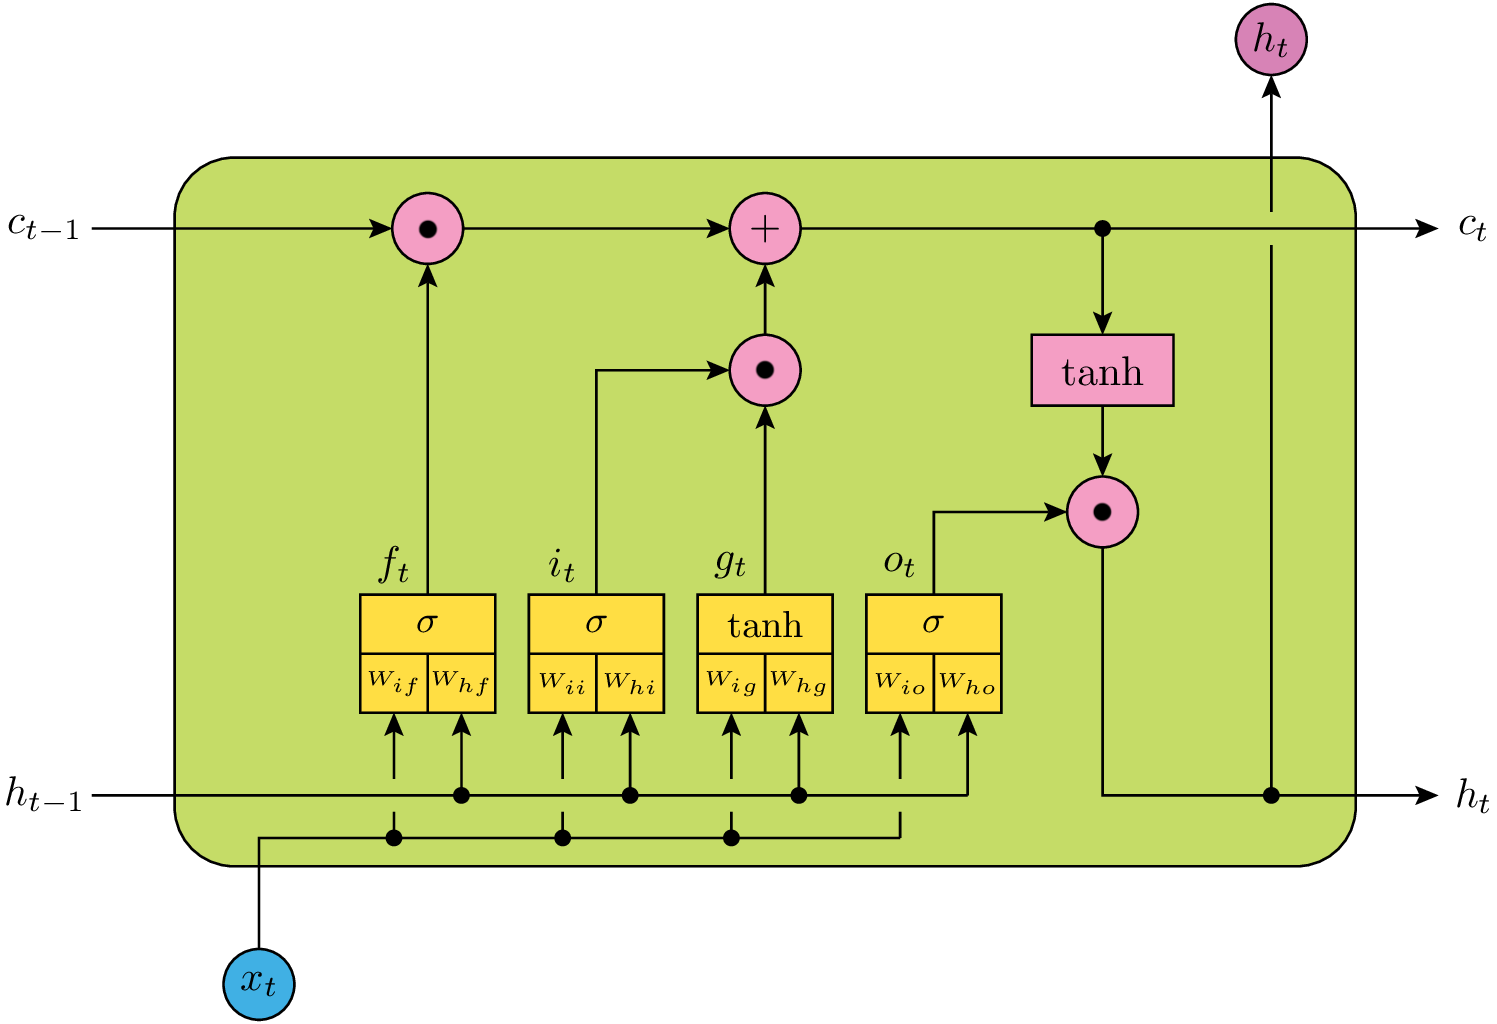
\includegraphics[width=10cm]{lstm_cell.png}
    \caption{LSTM cell \cite{lstmcell_img}}
    \label{fig:lstmCell}
\end{figure}

\subsubsection{Bidirectional Long Short-Term Memory}

Similarly, as previously described in BRNN (1.2.3.1), Bidirectional Long Short-Term Memory (BLSTM) has its hidden state split into two, forward states and backward states. Such modification allows the network to gain context from past and future alike. As a result, BLSTM, in comparison with BRNN, handles better the information storage across the timeline with large time gaps from either past or future.

\begin{figure}[h]
    \centering
    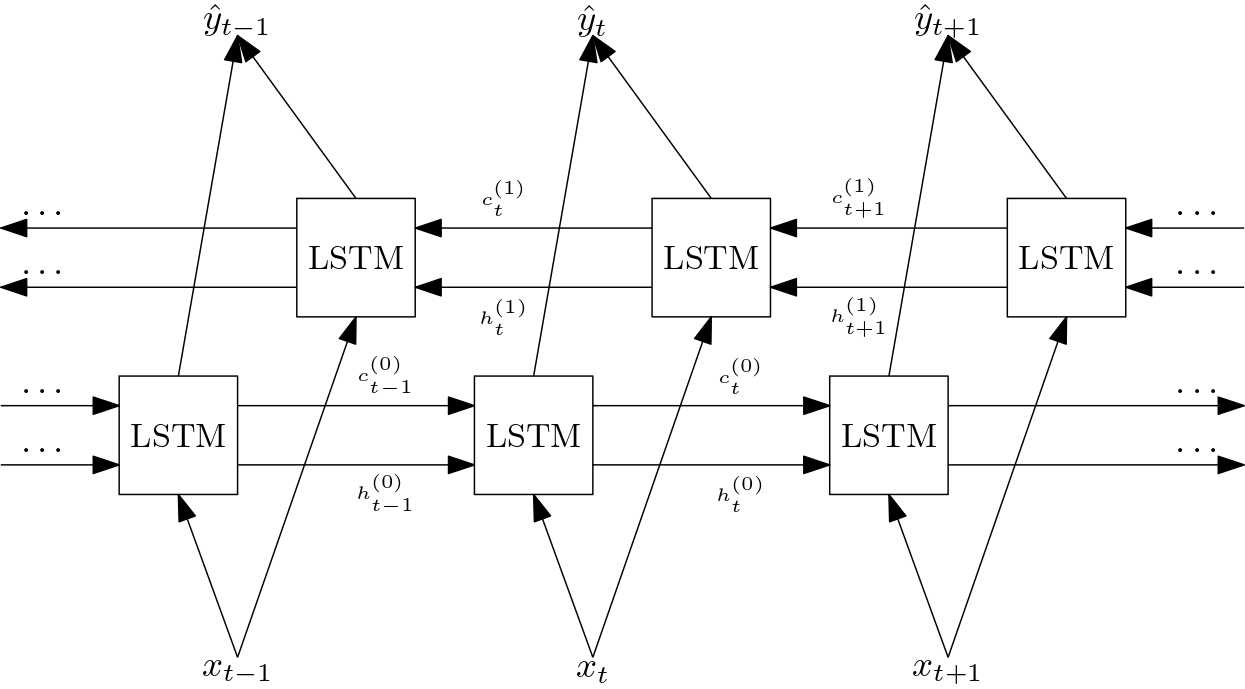
\includegraphics[width=12cm]{lstm_bi.png}
    \caption{Unrolled structure of BLSTM \cite{matous}}
    \label{fig:blstm}
\end{figure}

\subsubsection{Deep Long Short-Term Memory}

Deep Long Short-Term Memory (DLSTM), or stacked LSTM, is now considered a stable technique for challenging sequence prediction tasks. It was first introduced by Graves et al. \cite{gravesDLSTM}, where it was found that the depth of the network has greater importance than the number of memory cells in a given layer. Thus, DLSTM architecture can be described as an LSTM model consisting of multiple LSTM layers.

\begin{figure}[H]
    \centering
    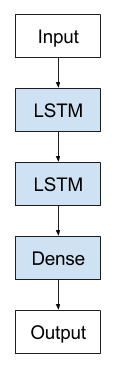
\includegraphics[width=3cm]{dlstm.png}
    \caption{Deep Long Short-Term memory architecture \cite{brownleeDLSTM}}
    \label{fig:dlstm}
\end{figure}

The LSTM layer above outputs a sequence rather than a single value for the LSTM layer below \cite{brownleeDLSTM}.

